\section{Classification of items and bins}

We take an instance with an optimal packing into $m$ bins of size at
most 12 and, assuming that our algorithm fails, we derive a
contradiction. One way to get a contradiction is to show that the size
of all items is larger than $12m$. As stated above, 
we also use two bounds in the
spirit of weight functions: weight $w(i)$ and value $v(i)$. The weight
$w(i)$ is a slightly modified size to account for items of size larger
than 6. The value $v(i)$ only counts the number of items with
relatively large sizes. For our calculations, it is convenient to
normalize the weight $w(i)$ and value $v(i)$ so that they are at most
0 for bins in the optimal packing (see Lemma~\ref{l:weight}). To get a contradiction, it is then sufficient to prove that
the total weight or value of all bins is positive.

\subsection{Classification of items}

We classify the items based on their size $s(i)$ and define their
value $v(i)$ as follows.  
$$
\begin{array}{c|cccc}
s(i) & (9,12] &(6,9] &(3,4] &(0,3]\cup(4,6]\\
\hline\\[-0.9em]
\mbox{~~type~~} & \mbox{~~huge~~} &\mbox{~~large~~} &\mbox{~~medium~~} &\mbox{~~regular~~}\\
v(i) & 3 & 2 & 1 & 0
\end{array}
$$

\begin{dfn}
For a set of items $A$, we define the value $v(A)=(\sum_{i\in
  A}v(i))-3$.

Furthermore we define weight $w(A)$ as follows. Let $k(A)$ be the
number of large and huge items in $A$. Then $w(A)=s(A)+k(A)-13$.

For a set of bins $\calA$ we define $v(\calA)=\sum_{A\in\calA}v(A)$,
$w(\calA)=\sum_{A\in\calA}w(A)$ and $k(\calA)=\sum_{A\in\calA}k(A)$.
\end{dfn}

\begin{lem}
\label{l:weight}
For any packing $\calA$ of a valid input instance into $m$ bins of an
arbitrary capacity,
we have $w(\calA)\leq 0$ and $v(\calA)\leq 0$.
\end{lem}
\begin{proof}
For the value $v(\calA)$, no optimal bin can contain items
with the sum of their values larger than 3. The bound follows by
summing over all bins and the fact that the number of bins is the same
for the optimum and the considered packing. 

For $w(\calA)$, we have $s(\calA)\leq 12m$ and $k(\calA)\leq m$, as the
optimum packs all items in $m$ bins of volume $12$ and no bin can
contain two items larger than $6$. Thus
$w(\calA)=s(\calA)+k(\calA)-13m\leq 12m+m-13m=0$.
% \qed
\end{proof}

\begin{figure}[th]
\begin{center}
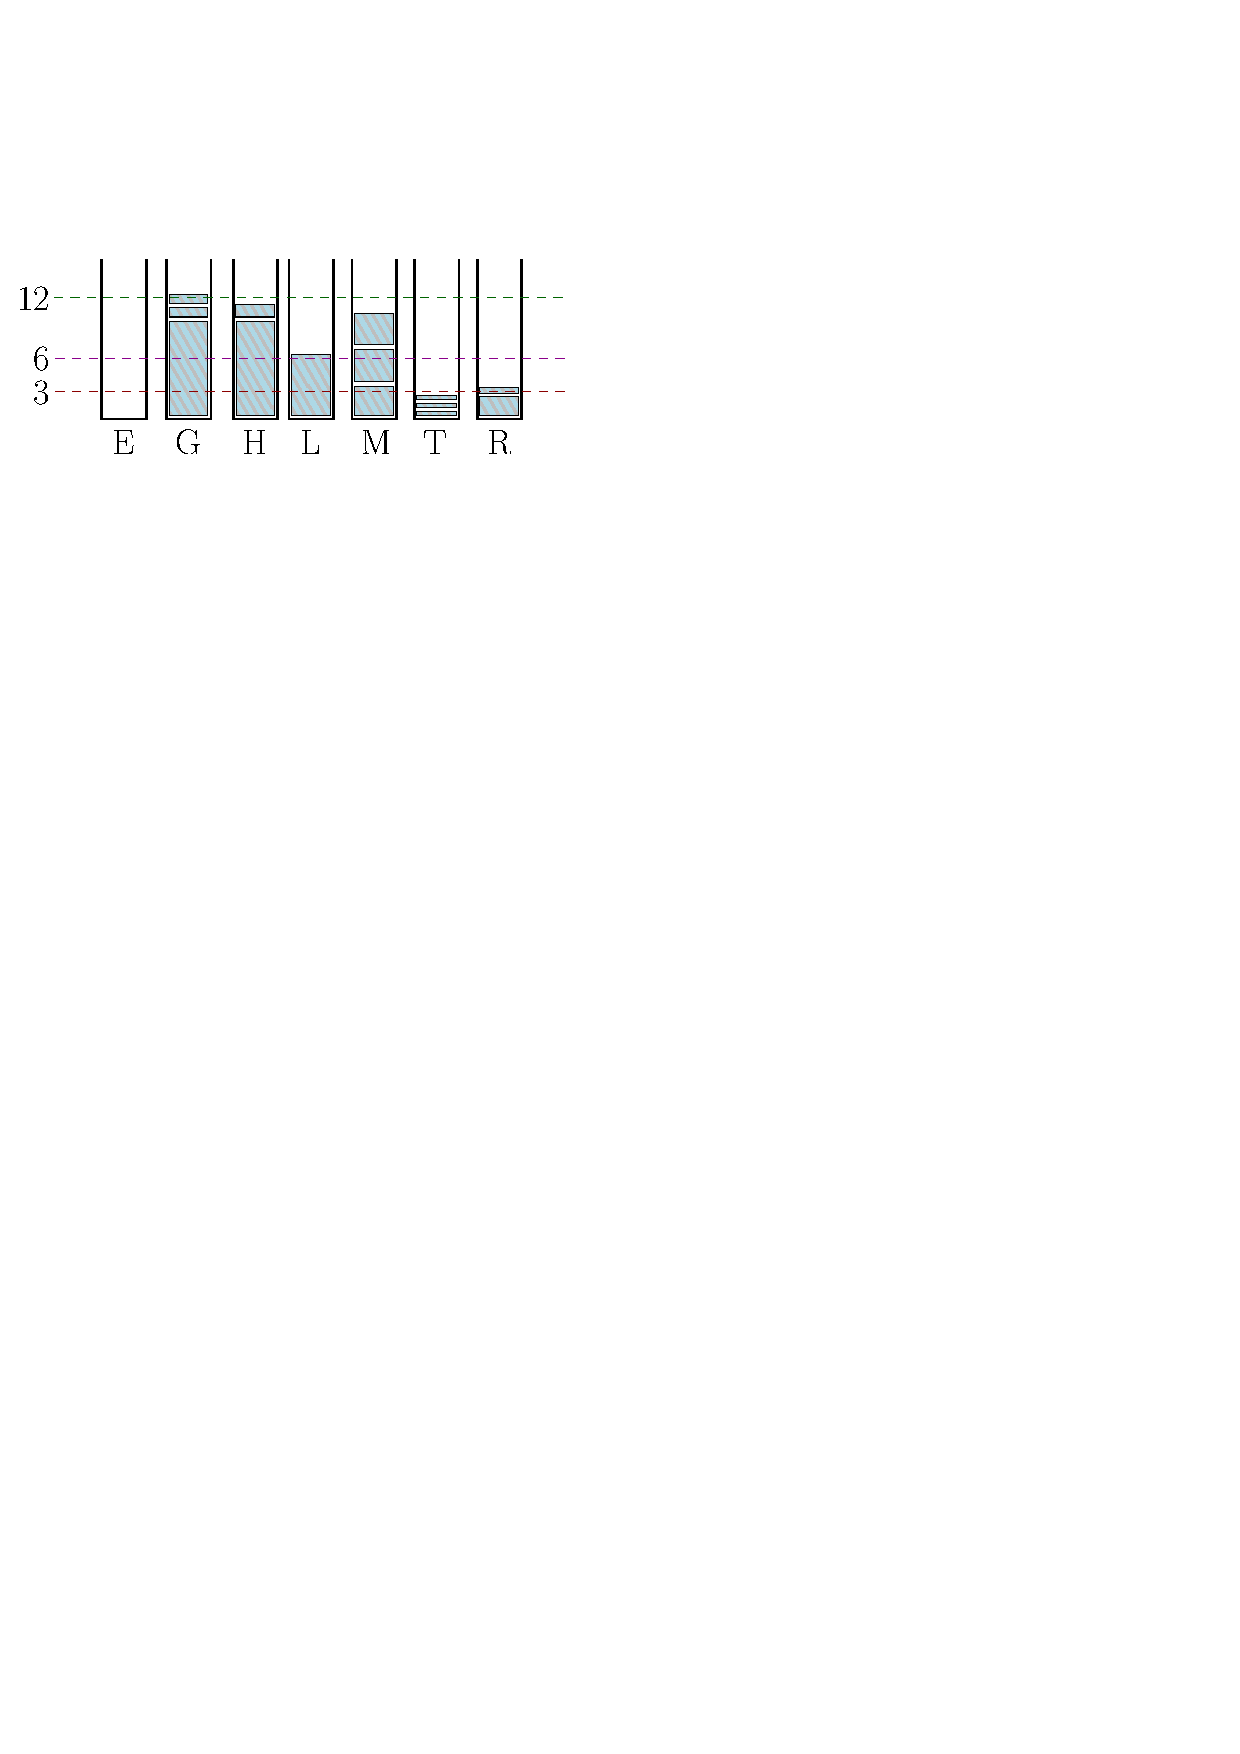
\includegraphics[width=0.7\textwidth]{img/bin_types.pdf}
\end{center}
\caption{An illustration of bin types during the first phase.}
\label{fig:1a}
\end{figure}
%

% \noindent{\bf First phase.}

\subsection{Classification of bins}

Along with items of specific types, we also wish to classify bins
based on which types of items they contain as well as other properties
(load, weight, value).

While item types are persistent, bin types change as items are added
to the bins. As mentioned, our algorithm will work in two phases, and
we make use of the bin types only during the first phase and when
transitioning into the second phase.

During the first phase, our algorithm maintains the invariant that
only bins of certain types exist, namely those from
Definition~\ref{d:types}. See Figure~\ref{fig:1a} for an illustration
of these types.

\begin{dfn}\label{d:types}
Given a bin $A$, we define the following bin types and introduce
letters that typically denote those bins:

\begin{compactitem}
\item 
{\bf Empty bins (E):} bins that have no item.
\item 
{\bf Complete bins (G):} all bins that have $w(A)\geq 0$ and $s(A)\geq
12$;
\item 
{\bf Huge-item bins (H):} all bins that contain a huge item (plus possibly some other items) and have $s(A)<12$;
\item 
{\bf One large-item bin (L):} a bin containing only a single large
item;
\item 
{\bf One medium-item bin (M):} a non-empty bin with $s(A)<13$ and only medium
items;
\item 
{\bf One tiny bin (T):} a non-empty bin with $s(A)\leq3$;
\item 
{\bf Regular bins (R):} all other bins with $s(A)\in(3,6]$;
\end{compactitem}
\end{dfn}

